\chapter{SYSTEM ARCHITECTURE} \label{chap_sys_architecture}
System architecture is explained and analyzed under three sub sections.
\begin{enumerate}
    \item Main overview of the system is explained in the Section \ref{sec_overview_sys_architecture}.
    \item Hardware design and architecture is explained in the Section \ref{sec_hardware_design}.
    \item Firmware design and architecture is explained in the Section \ref{sec_firmware_design}
    \item SİLİNECEK \cite{One, Two, Three}.
    
\end{enumerate}

\section{Overview of the System Architecture} \label{sec_overview_sys_architecture}

The system consist of paired RC car and Android phone. Android phone, which runs the remote control interface, connects the target RC car unit via Bluetooth communication and send / receive control packets over this channel. At server (database) side, each Android\texttrademark\;phone connects to the Firebase database in order to establish an online session for game. Figure \ref{fig:overview_architecture} shows the diagram of the main system architecture.

\begin{figure}[!htbp]
    \centering
    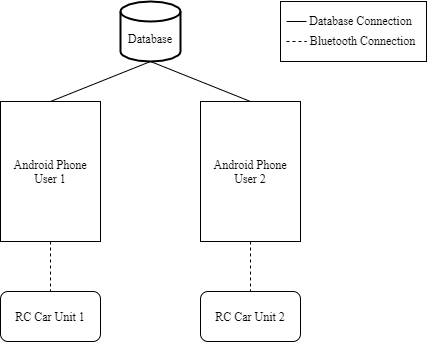
\includegraphics[width=0.8\textwidth]{Imgs/overview_of_sys.drawio.png}
    \caption{\label{fig:overview_architecture}Diagram of the Main System Architecture}
\end{figure}

\section{Hardware Design} \label{sec_hardware_design}

\subsection{Hardware Architecture} \label{sec_hardware_architecture}

Main hardware architecture and power / harness diagram is shown in Figure \ref{fig:hardware_architecture}. 

\begin{figure}[!htbp]
    \centering
    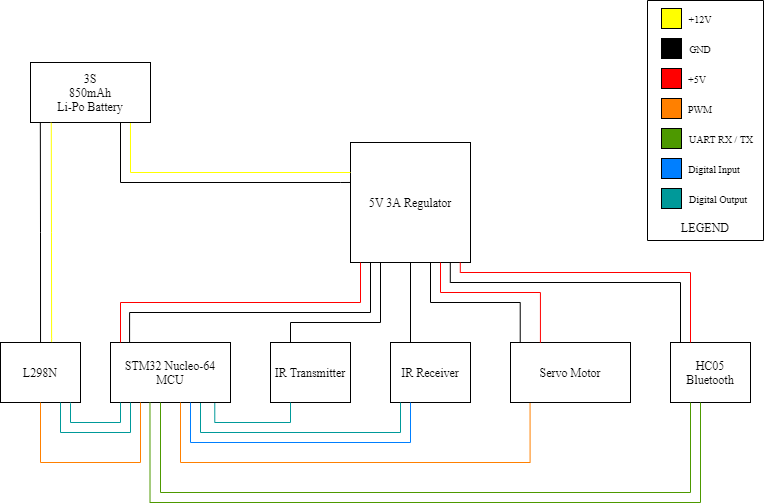
\includegraphics[width=1\textwidth]{Imgs/ana_devre_v3.png}
    \caption{\label{fig:hardware_architecture}Power / Harness Diagram of the Hardware}
\end{figure}

All system is powered from 3S 25C 850mAh Li-Po battery. This Li-Po battery can supply maximum current about 20A (C x mAh). This current capacity is enough for the supplying the system components. HC05 module, STM32 MCU and servo motor powered from the regulator output. This voltage regulator is a step down voltage regulator that decreases the voltage to 5V and supplies maximum 3A current.\\

L298N motor driver controlled by 3 input pins. 2 of these three input pins are controlling the direction of the DC motor. MCU writes digital output to these pins in order to change direction of the DC motor or completely stop the DC motor of the RC car unit. Other pin used for controlling the DC motor speed, by applying PWM signal to enable pin of the L298N motor driver. \\

Steering of the RC car controlled by the servo motor. This steering servo motor powered from voltage regulator 5V output and controlled from PWM signal that is generated by MCU of the RC car unit. \\

HC05 Bluetooth\texttrademark\;module connected to the UART pins of the MCU of the RC car unit. UART baud rate has been configured at 115200. HC05 RX pin is connected to the UART TX pin of the MCU, HC05 TX pin is connected to the UART RX pin of the MCU. By this way, MCU of the RC car unit communicate over the Bluetooth\texttrademark. \\

IR receiver is connected to the MCU of the RC car unit as a digital input in order to keep track of the hitting by the IR transmitter (led) coming from opponents RC car. IR transmitter (led) is connected to the MCU of the RC car unit as a digital input. By this way, IR transmitter (led) can be powered with GPIO pin whenever user wants.


% Hardware Components Part Start
\subsubsection{STM32 MCU}
The system uses STM32 Nucleo-64 development board as a MCU of the RC car unit. STM32 Nucleo-64 development board is based on processor Arm\textregistered\;Cortex\textregistered\;M4, has 32.768 kHz crystal oscillator,  has 11 timers: up to six 16-bit, two 32-bit timers up to 100 MHz, has 512 Kbytes of flash memory and 128 Kbytes of SRAM \cite{One}. This MCU provides necessary peripherals and clock speed for the RC car unit. This board has built-in ST link programming interface and driver which provides fast development without additional ST link device. The implementation of the hardware and firmware is not restricted with this development board, similar approach can be applied with any MCU that is based on Arm\textregistered\;Cortex\textregistered\;M4 family and that has sufficient number of timers, GPIOs and other essential peripherals. This development board is shown in Figure \ref{fig:nucleo64_board}.\\

\begin{figure}[!htbp]
    \centering
    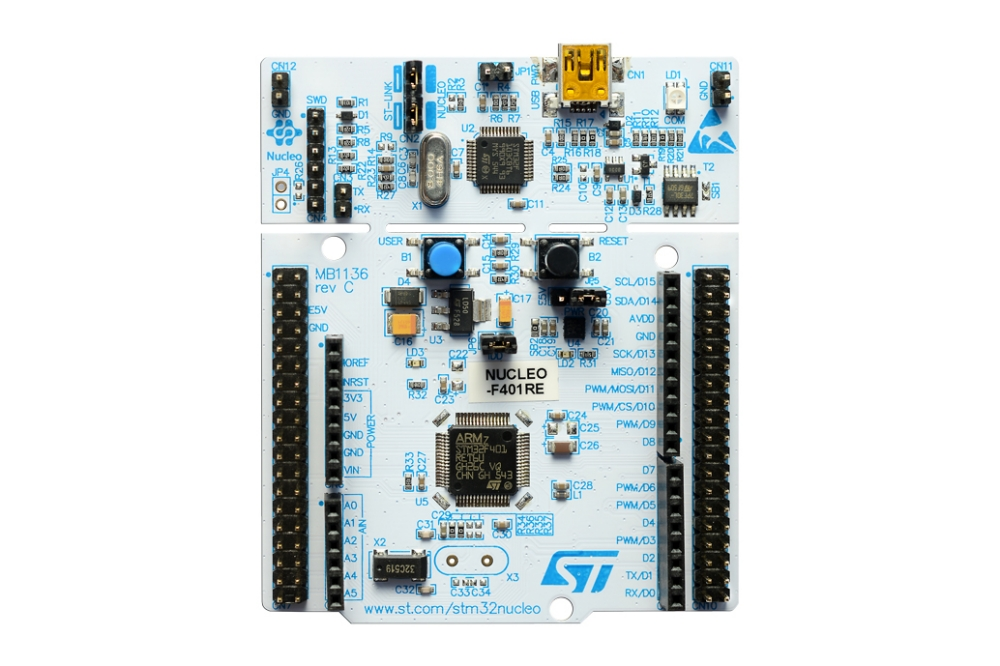
\includegraphics[width=0.9\textwidth]{Imgs/nucleo64.jpg}
    \caption{\label{fig:nucleo64_board}STM32 Nucleo-64 Development Board \cite{One}}
\end{figure}

\subsubsection{L298N DC Motor Driver}
STMicroelectronics\texttrademark\;L298N dual full bridge DC motor driver is used for driving the DC motor of the RC car unit. It is a high voltage, high current dual full-bridge driver designed to accept standard TTL logic levels and drive inductive loads such as relays, solenoids, DC and stepping motors. Two enable inputs are provided to enable or disable the device independently of the input signals. This enable inputs accepts PWM signals for driving motors with speed control. The L298N motor driver accepts 5-46V supply, provides maximum 2A DC current per channel \cite{Two}. According to these specifications and power ratings, this motor driver meets the requirements of the RC car unit. Motor driver PCB is show in Figure \ref{fig:l298n_pcb} .

\begin{figure}[!htbp]
    \centering
    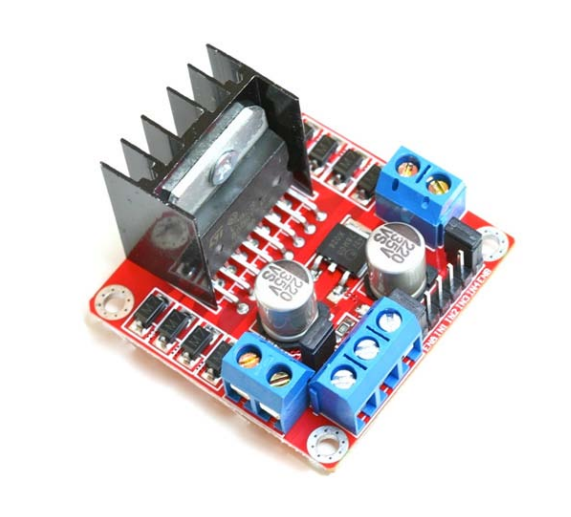
\includegraphics[width=0.5\textwidth]{Imgs/l298n.png}
    \caption{\label{fig:l298n_pcb}L298N Motor Driver PCB}
\end{figure}

\subsubsection{Servo Motor}
Servo motors have rapid acceleration and deceleration and provides high torques for many mechanic applications with allowing position control. High dynamic response and precision make them suitable for motion control applications and robotics. In the RC car unit, servo motor used for steering. Thus, precise steering control can be achieved.\\

In this project, TowerPro\texttrademark\; MG90S servo motor used. This servo motor works at 4.8V - 6V and has 1.8kg/cm stall torque. Maximum stall current consumption is about 1A \cite{Ref_servo_mg90s}. According to these running and power specifications, this servo motor meets the requirements of the RC car unit.


\subsubsection{Voltage Regulator}
LM2596 3A Step-Down Voltage Regulator is used for powering the system components which accept 5V for supply voltage. MCU, servo motor and HC05 Bluetooth\texttrademark\;module are powered from voltage regulator output. The LM2596 series of regulators are monolithic
integrated circuits that provide all the active functions for a step-down (buck) switching regulator, capable of driving a 3-A load with excellent line and load
regulation \cite{Three}. This voltage regulator supplies enough output current for powering the 5V components in the system.

\subsubsection{HC05 Bluetooth Module} \label{sec_hc05_module}
The Bluetooth\texttrademark\;wireless technology is designed as a short-range networking solution for personal, portable electronic devices and embedded systems. It overcomes the limitations of line of sight and one to one communication of its possible competitor Infra-Red(IR). It operates in the 2.4 GHz Industrial, Scientific and Medical (ISM) band at a maximum data rate of 720 Kbps \cite{Bluetooth_Overview}. \\

In RC Car Battle system, Bluetooth\texttrademark\;is used for communication between the RC car unit and the remote controller Android\texttrademark\;phone. HC05 Bluetooth\texttrademark\;module used for adding Bluetooth\texttrademark\;interface to the STM32 MCU of the system. HC05 module is Bluetooth SPP (Serial Port Protocol) module, designed for transparent wireless serial connection setup. It has integrated antenna and programmable UART interface. Baud rate, password, name of the can be configured over this UART interface in configuration mode \cite{HC05_datasheet}. This module allows MCU to communicate with Bluetooth\texttrademark\;over the UART interface. 115200 baud rate used for UART communication with the HC05 module. This module is shown in Figure \ref{fig:hc05_module}. \\ 

\begin{figure}[!htbp]
    \centering
    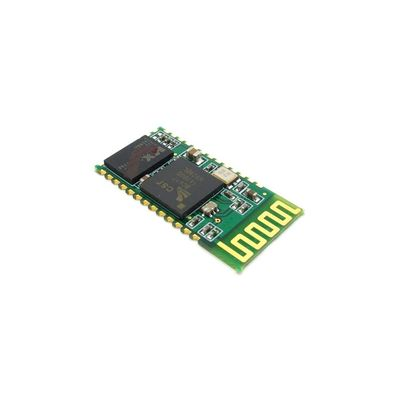
\includegraphics[width=0.5\textwidth]{Imgs/400px-HC-05.jpg}
    \caption{\label{fig:hc05_module}HC05 Bluetooth\texttrademark\; Module \cite{HC05_datasheet}}
\end{figure}

\subsubsection{IR Transmitter and Receiver Module}
The RC car units simulates the shooting and hitting by IR transmitter (IR Led) and IR receiver module which. Keyestudio\texttrademark\;infrared obstacle avoidance sensor (IR-08H) used for achieving this functionality. Main purpose of this module is estimating distance by using IR led and IR receiver for obstacle avoidance applications on robotic systems. It has a pair of infrared transmitting and receiving tube. When infrared ray launched by the transmitting tube encounters an obstacle (its reflector), the infrared ray is reflected to the receiving tube, and the indicator will light up; the signal output interface outputs digital signal. This module works at DC 3.3V-5V voltage values. The logic level 3.3V and power consumption ratings are compatible with the MCU of the RC car unit.\\

IR transmitter and receiver module has been modified for this project. A RC car unit has two of this IR module, one for transmitter which is on front side of the RC car, one for receiving IR light which is on back side of the RC car. IR receiver part removed from the transmitter IR module. IR transmitter (led) part removed from the receiver IR module. 

% Hardware Components Part End

\subsection{RC Car Control Unit}
In this project, custom RC car control unit has been designed on PCB. The designed and developed multi-layered PCB gathers system components under a single circuit. The PCB contains female and male headers for system components. The motivation behind the design and produce PCB is avoid short circuit and loose electrical connections. The RC car control unit provides robust connection between system components and electronic modules. The designed PCB contains the following system component connections :
\begin{enumerate}
    \item Servo and DC motor male header pins.
    \item HC05 Bluetooth\texttrademark\;female header pins.
    \item STM32 MCU female header pins.
    \item Voltage regulator pad connections.
    \item L298N motor driver pad connections.
    \item Voltage divider circuit, resistor connections.
    \item Input power male header pins.
    \item Jumper for selecting the Li-Po battery ADC input with male headers.
    \item UART male header pins for debugging.
\end{enumerate}


\begin{figure}[!htbp]
    \centering
    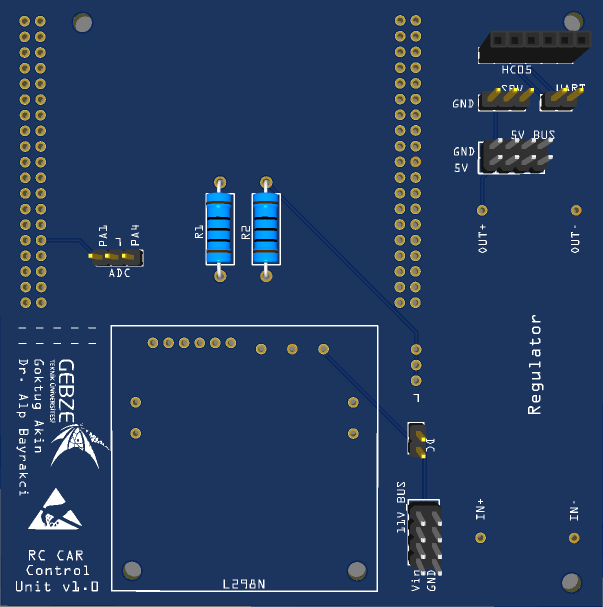
\includegraphics[width=0.75\textwidth]{Imgs/pcb.png}
    \caption{\label{fig:custom_pcb}Design View of RC Car Control Unit PCB}
\end{figure}

asd
The Algorithm \ref{labelOfAlgorithm} shows the pseudo code of...
\begin{algorithm}
\caption{Caption of the algorithm}
\label{labelOfAlgorithm}
\begin{algorithmic}
\Require $n \geq 0$ % i.e. input
\Ensure $y = x^n$  % i.e. output
\State $y \gets 1$
\State $X \gets x$
\State $N \gets n$
\While{$N \neq 0$}
\If{$N$ is even}
    \State $X \gets X \times X$
    \State $N \gets \frac{N}{2}$  \Comment{This is a comment}
\ElsIf{$N$ is odd}
    \State $y \gets y \times X$
    \State $N \gets N - 1$
\EndIf
\EndWhile
\end{algorithmic}
\end{algorithm}

\section{Firmware} \label{sec_firmware_design}

\subsection{Bidirectional Reliable Bluetooth Communication} \label{sec_bluetooth_comm}

Communication with the controller smartphone and the RC car unit provided via Bluetooth\texttrademark.\;Hardware details of the Bluetooth\texttrademark\;explained in the Section \ref{sec_hc05_module}. This section explains the implementation details of the bidirectional Bluetooth\texttrademark\; communication.

\subsubsection{Receiving RC Command From Smartphone} \label{sec_receive_rc_command}

The remote controller smartphone sends RC command to the target RC car unit at 10 HZ. HC05 module receives the incoming data from the controller smartphone, and sends these incoming data to the UART peripheral of MCU of the RC car unit. This communication runs at 115200 baud-rate. \\

The UART unit of the STM32 MCU generates IRQ when new data available on the UART line. Custom ISR has been implemented for catching and handling the interrupts. The UART interrupts used for efficient communication instead of polling method in order to avoid consuming unnecessary cycles. UART line is authorized in the NVIC unit of the MCU for an interrupt to occur from the UART unit of the MCU. \\

To able the enabling the read interrupts from the UART unit, RXNEIE (RX not empty interrupt enabled) bit of the CR1 (Control Register 1) has been set to 1. After this configuration, when there is a data to be read on the UART line, an interrupt will be generated from the UART unit. This control register is shown in Figure \ref{fig:uart_cr_register}. RXNEIE bit of the register highlighted in yellow.

\begin{figure}[!htbp]
    \centering
    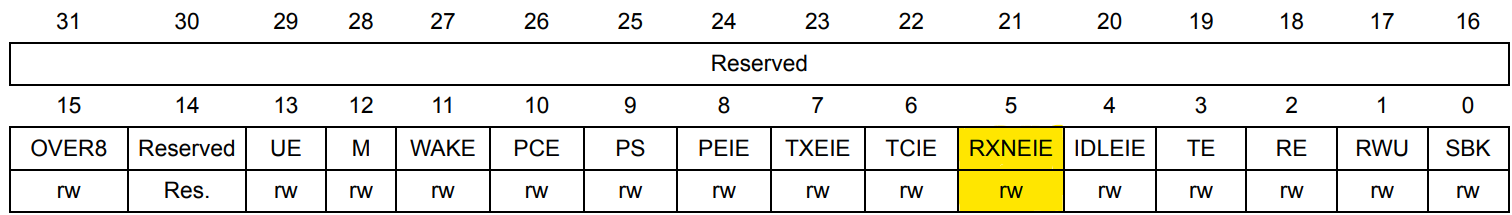
\includegraphics[width=1\textwidth]{Imgs/cr_register.png}
    \caption{\label{fig:uart_cr_register}UART Control Register 1 of the MCU (REFERANS VERILMELI USAR MANUAL)}
\end{figure}



\subsubsection{Transmitting RC Car Information to the Smartphone}
\label{sec_transmit_rc_info}


\subsection{Controlling Motors} \label{sec_controlling_motors}

\subsection{IR Receiver and IR Transmitter} \label{sec_ir_rx_tx}

\subsection{Reading Li-Po Battery Voltage} \label{sec_read_lipo_voltage}

\subsection{Main Overview of the System Components} \label{main_system_components}

\section{Remote Controller Application} \label{sec_remote_app}

\subsection{User Interface} \label{sec_user_interface}

\subsection{RC Car Communication} \label{sec_rc_comm}

\subsection{Database Connection} \label{sec_db_connection}



\begin{comment}
% Below are comments, just for source..
    Ut enim ad minima veniam, quis nostrum exercitationem ullam corporis suscipit laboriosam, nisi ut aliquid ex ea commodi consequatur? Quis autem vel eum iure reprehenderit qui in ea voluptate velit esse quam nihil molestiae consequatur, vel illum qui dolorem eum fugiat quo voluptas nulla pariatur? \ref{tab:widgetss}

    \begin{table}[!htbp]
    \centering
    \caption{\label{tab:widgetss}Comparison of percentages.}
    \begin{tabular}{c|cc|cc}
    \hline
    Mode &  \multicolumn{2}{c}{Var} & \multicolumn{2}{c}{Cum}\\ 
    \hline
    1   &  17.5 & 19.1   & 17.5  & 19.1\\
    2   &  11.8 & 12.7   & 29.3  & 31.9\\
    3   &  6.6  &  5.6   & 35.9  & 37.4\\
    \end{tabular}
    \end{table}
    
    \begin{enumerate}
    \item first,
    \item second.
    \end{enumerate}
    \dots and bullet points \dots
    \begin{itemize}
    \item one bullet,
    \item two bullets.
    \end{itemize}
    
    Let $X_1, X_2, \ldots, X_n$ be a sequence of independent and identically distributed random variables with $\text{E}[X_i] = \mu$ and $\text{Var}[X_i] = \sigma^2 < \infty$, and let
    \[S_n = \frac{X_1 + X_2 + \cdots + X_n}{n}
          = \frac{1}{n}\sum_{i}^{n} X_i\]
    denote their mean. Then as $n$ approaches infinity, the random variables $\sqrt{n}(S_n - \mu)$ converge in distribution to a normal $\mathcal{N}(0, \sigma^2)$.
    
    \begin{quote}
        At vero eos et accusamus et iusto odio dignissimos ducimus qui blanditiis praesentium voluptatum deleniti atque corrupti quos dolores et quas molestias excepturi sint occaecati cupiditate non provident, similique sunt in culpa qui officia deserunt mollitia animi, id est laborum et dolorum fuga.
    \end{quote}
\end{comment}